\documentclass[12pt,a4paper]{article}
\usepackage{amsmath,amscd,amsbsy,amssymb,latexsym,url,bm,amsthm}
\usepackage{epsfig,graphicx,subfigure}
\usepackage{enumitem,balance}
\usepackage{wrapfig}
\usepackage{mathrsfs,euscript}
\usepackage[usenames]{xcolor}
\usepackage{hyperref}
\usepackage[vlined,ruled,linesnumbered]{algorithm2e}
\usepackage{float}
\hypersetup{colorlinks=true,linkcolor=black}

\newtheorem{theorem}{Theorem}
\newtheorem{lemma}[theorem]{Lemma}
\newtheorem{proposition}[theorem]{Proposition}
\newtheorem{corollary}[theorem]{Corollary}
\newtheorem{exercise}{Exercise}
\newtheorem*{solution}{Solution}
\newtheorem{definition}{Definition}
\theoremstyle{definition}

\renewcommand{\thefootnote}{\fnsymbol{footnote}}

\newcommand{\postscript}[2]
 {\setlength{\epsfxsize}{#2\hsize}
  \centerline{\epsfbox{#1}}}

\renewcommand{\baselinestretch}{1.0}

\setlength{\oddsidemargin}{-0.365in}
\setlength{\evensidemargin}{-0.365in}
\setlength{\topmargin}{-0.3in}
\setlength{\headheight}{0in}
\setlength{\headsep}{0in}
\setlength{\textheight}{10.1in}
\setlength{\textwidth}{7in}
\makeatletter \renewenvironment{proof}[1][Proof] {\par\pushQED{\qed}\normalfont\topsep6\p@\@plus6\p@\relax\trivlist\item[\hskip\labelsep\bfseries#1\@addpunct{.}]\ignorespaces}{\popQED\endtrivlist\@endpefalse} \makeatother
\makeatletter
\renewenvironment{solution}[1][Solution] {\par\pushQED{\qed}\normalfont\topsep6\p@\@plus6\p@\relax\trivlist\item[\hskip\labelsep\bfseries#1\@addpunct{.}]\ignorespaces}{\popQED\endtrivlist\@endpefalse} \makeatother

\begin{document}

\noindent

%========================================================================
\noindent\framebox[\linewidth]{\shortstack[c]{
\Large{\textbf{Lab04-Matroid}}\vspace{1mm}\\
CS214-Algorithm and Complexity, Xiaofeng Gao, Spring 2021.}}
\begin{center}
\footnotesize{\color{red}$*$ If there is any problem, please contact TA Haolin Zhou.}

% Please write down your name, student id and email.
\footnotesize{\color{blue}$*$ Name: WendiChen  \quad Student ID: 519021910071 \quad Email: chenwendi-andy@sjtu.edu.cn}
\end{center}

\begin{enumerate}
\item \textit{Property of Matroid.} 
\begin{enumerate}
	\item
	Consider an arbitrary undirected graph $ G=(V,E) $. Let us define $ M_{G}=(S,C) $ where $ S=E $ and $ C=\left\{I \subseteq E \mid\left(V, E \backslash I\right) \text { is connected}\right\} $. Prove that $ M_{G} $ is a \textbf{matroid}.\par
	\begin{solution}
	 ~\\
	 Let us prove \emph{Hereditary} first.\\
	 If $B$ satisfies that $B\in C$ and $(V,E\backslash B)$ is connected, for any $A\subset B$, we have $E\backslash B \subset E\backslash A$.
	 Therefore, $(V,E\backslash A)$ is also connected and $A \in C$.\\
	 Then we'll prove the \emph{exchange property}. \\
	 Consider $A,B \in C$ with $|A|<|B|$. Note that $(V,E\backslash B)$ is connected, then $|E\backslash B|\ge n-1$. Thus, we have $|E\backslash A|>|E\backslash B|\ge n-1$.
	 That implies $(V,E\backslash A)$ has at least one circle.
	 And there must exist one edge $e$ on one circle of $(V,E\backslash A)$ which is not involved in $(V,E\backslash B)$(if not, all circles in $(V,E\backslash A)$ exist in $(V,E\backslash B)$, which means $|E\backslash A|\leq|E\backslash B|$ and contradicts).
	 Thus, we have $e\in B\backslash A$ and $(V,E\backslash (A\cup \{e\}))$ is connected. Therefore, $E\backslash (A\cup \{e\}) \in C$.\\
	 Thus, we successfully prove that $M_G$ is a matroid.
	 \begin{figure}[htbp]
        \centering
        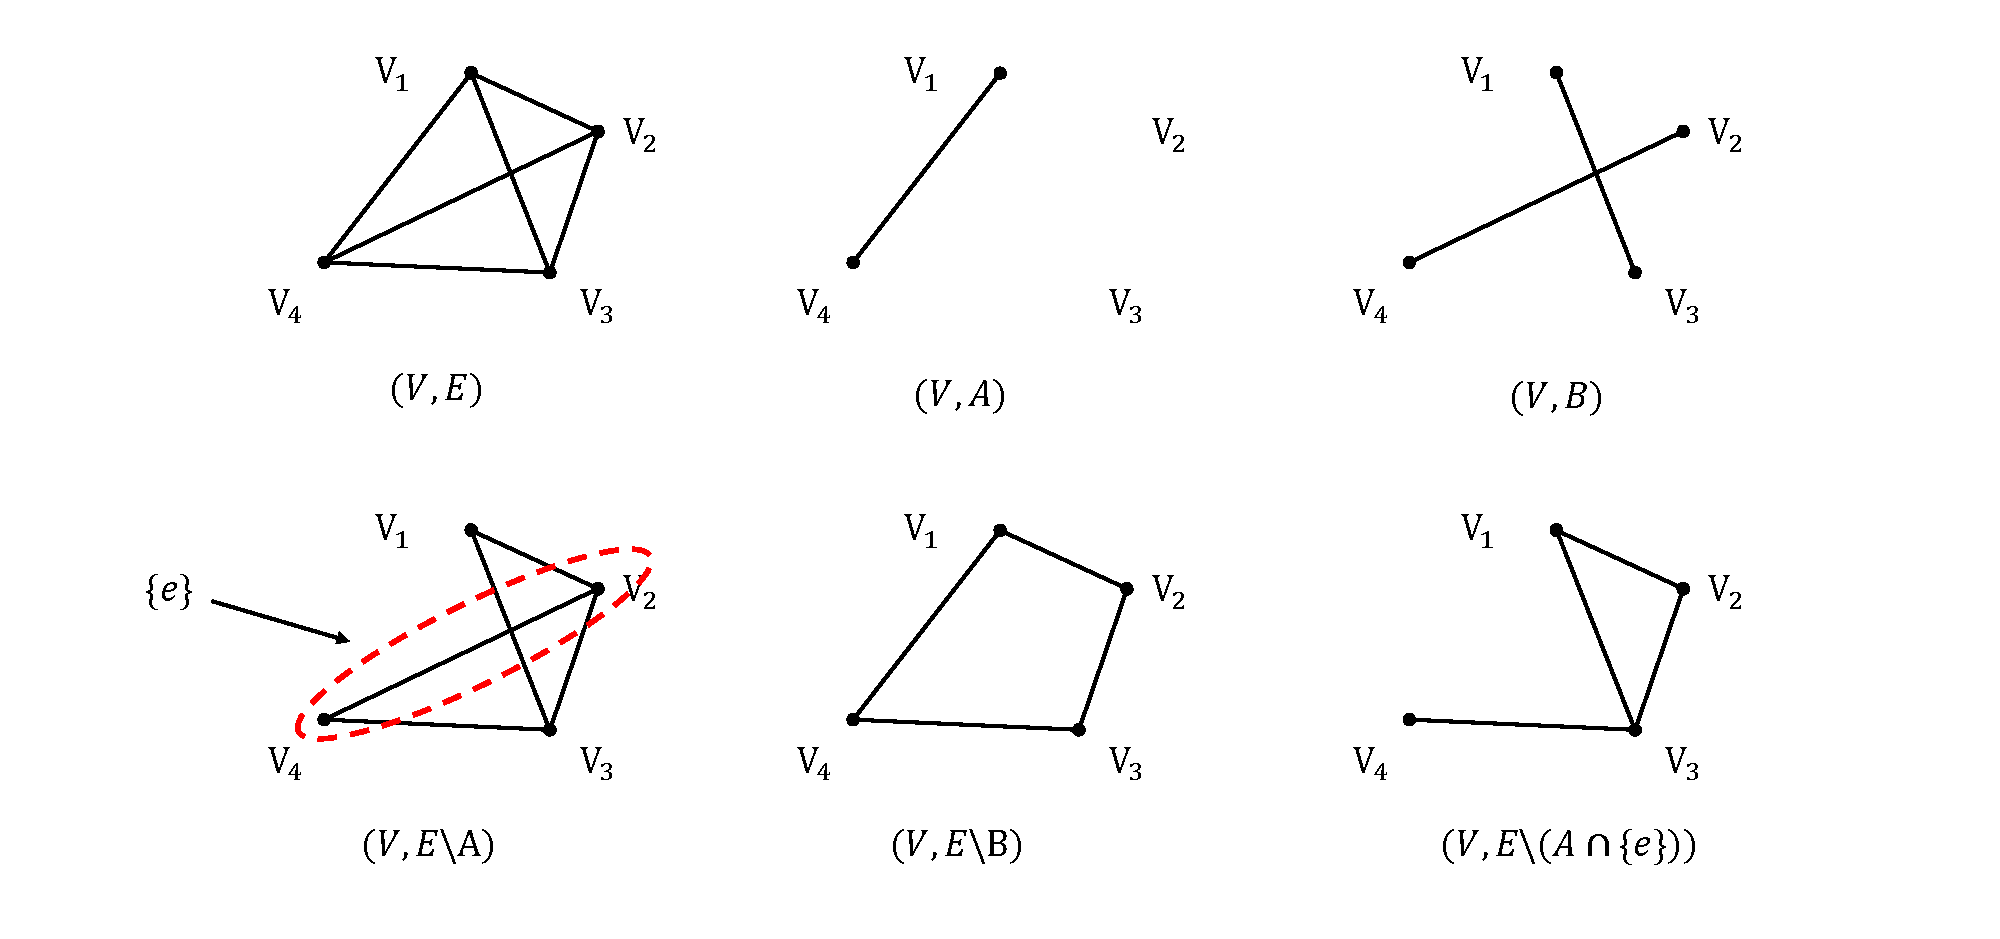
\includegraphics[width=0.9\textwidth]{Fig-CographicMatroid.pdf}
        \caption{Proof for Cographic Matroid}\label{Fig-Cographic}
    \end{figure}
    
	\end{solution}
	\item
	Given a set $A$ containing $n$ real numbers, and you are allowed to choose $k$ numbers from $A$. The bigger the sum of the chosen numbers is, the better. What is your algorithm to choose? Prove its correctness using \textbf{matroid}.\par
	\textbf{Remark:} Denote $\mathbf{C}$ be the collection of all subsets of $A$ that contains no more than $k$ elements. Try to prove $(A,\mathbf{C})$ is a matroid.\par
	\begin{solution}
	~\\
	\item 
	    \begin{minipage}[t]{0.8\textwidth}
        \begin{algorithm}[H]
        \KwIn{A set $A$ containing $n$ real numbers and an integer $k$}
        \KwOut{A set of $k$ numbers which has the biggest sum}
        		
        \BlankLine
        \caption{Greedy Algorithm to Choose $k$ Numbers}
        \label{greedy-choose}
        Sort all $n$ numbers in $S$ into ordering $x_1\ge x_2\ge \dots \ge x_n$\;
        $A\leftarrow \emptyset$\;
        \For{$i = 1 \text{ to } n$ }{
            \If{$A \cup\{x_i\} \in C$}{
                $A\leftarrow A \cup\{x_i\}$\;
            }
        }
        \Return $A$\;
        \end{algorithm}
        \end{minipage}
        
        As the remark described above, now we will prove that $(A,\mathbf{C})$ is a matroid.\\
        Let us prove \emph{Hereditary} first.\\
        If $B$ is a subset of $B$ which contains no more than $k$ elements, then for any $A\subset B$, $|A|<|B|\leq k$. Thus, $A\in \mathbf{C}$.\\
        Then we will prove the exchange property.\\
        Consider $A,B \in \mathbf{C}$ with $|A|<|B|$. There must exist one element $e$ satisfying $e\in B\backslash A$. Then $|A\cup\{e\}|\leq |B|\leq k$. Thus $A\cup \{e\}\in \mathbf{C}$.\\
        Therefore, we successfully prove that $(A,\mathbf{C})$ is a matroid. So, the Alg.\ref{greedy-choose} is actually the \emph{Greedy-MAX} algorithm, which performs an optimal solution for a matroid.
        
	\end{solution}

\end{enumerate}
\item \textit{Unit-time Task Scheduling Problem.} Consider the instance of the \textbf{Unit-time Task Scheduling Problem} given in class. 
    \begin{enumerate}
        \item Each penalty $\omega_{i}$ is replaced by $80-\omega_{i}$. The modified instance is given in Tab.~\ref{tab:1}. Give the final schedule and the optimal penalty of the new instance using Greedy-MAX.
		\begin{table}[H]
			\setlength{\abovecaptionskip}{0.cm}
			\setlength{\belowcaptionskip}{0.5cm}
			\centering
			\caption{Task}
			\label{tab:1}			
			\begin{tabular}{|c|ccccccc|}
				\hline
				$ a_{i} $&1&2&3&4&5&6&7\\
				\hline
				$ d_{i} $&4&2&4&3&1&4&6\\
                \hline
                $ \omega_{i} $&10&20&30&40&50&60&70\\
				\hline
			\end{tabular}
		\end{table}
	   \begin{solution}
	    ~\\
	    Firstly, we sort the tasks non-increasingly and get the table below
	    \begin{table}[H]
			\setlength{\abovecaptionskip}{0.cm}
			\setlength{\belowcaptionskip}{0.5cm}
			\centering
			\caption{Sorted Task}
			\label{tab:2}			
			\begin{tabular}{|c|ccccccc|}
				\hline
				$ a_{i} $&7&6&5&4&3&2&1\\
				\hline
				$ d_{i} $&6&4&1&3&4&2&4\\
                \hline
                $ \omega_{i} $&70&60&50&40&30&20&10\\
				\hline
			\end{tabular}
		\end{table}
		Then, we check whether $A\cup\{a_i\}\in \mathbf{C}$ for each $a_i$ in order. At last, the \emph{Greedy-MAX} selects $A = \{a_7,a_6,a_5,a_4,a_3\}$ and reject $a_2,a_1$. We sort $A$ non-decreasingly by $d_i$ and get the final schedule is $\langle a_5,a_4,a_3,a_6,a_7,a_1,a_2\rangle$. The optimal penalty is $\omega_1+\omega_2 = 30$.
	   \end{solution}
        \item Show how to determine in time $O(|A|)$ whether or not a given set $A$ of tasks is independent. (\textbf{Hint}: You can use the lemma of equivalence given in class)
 	    \begin{solution}
        ~\\
        According to the lemma of equivalence, we naturally introduce the the sum of prefixes to simply the process of judgement. We can simply calculate the number of each $d_i$ and then use the sum of prefixes to determine whether $A$ is independent. From Alg.\ref{judgement}, we can find that the time complexity is obviously $O(k) = O(|A|)$.
        
        \begin{minipage}[t]{0.8\textwidth}
        \begin{algorithm}[H]
        \KwIn{A set $A$ of $k$ tasks, where $A = \{x_1,\dots,x_k\}$}
        \KwOut{A boolean that implies whether $A$ is independent}
        		
        \BlankLine
        \caption{Algorithm to Determine the Independence of Set $A$}
        \label{judgement}
        $count[1,\dots, n]\leftarrow[0,\dots,0]$\;
        $prefix\leftarrow 0$\;
        \For{$i = 1 \text{ to } k$ }{
            $count[d_i]\leftarrow count[d_i]+1$\;
        }
        \For{$i = 1 \text{ to } k$ }{
            $prefix \leftarrow prefix + count[i]$\;
            \If{prefix>i}{
            \Return $False$\;
            }
        }
        \Return $True$\;
        \end{algorithm}
        \end{minipage}
        
    \end{solution}
    \end{enumerate}

\item \textit{MAX-3DM.} Let $X$, $Y$, $Z$ be three sets. We say two triples $\left(x_{1}, y_{1}, z_{1}\right)$ and $\left(x_{2}, y_{2}, z_{2}\right)$ in $X \times Y \times Z$ are \textit{disjoint} if $x_{1} \neq x_{2}$, $y_{1} \neq y_{2},$ and $z_{1} \neq z_{2}$. Consider the following problem:
    
    \begin{definition}[MAX-3DM] 
        Given three disjoint sets $X$, $Y$, $Z$ and a non-negative weight function $c(\cdot)$ on all triples in $X \times Y \times Z$, \textbf{Maximum 3-Dimensional Matching} (MAX-3DM) is to find a collection $\mathcal{F}$ of disjoint triples with maximum total weight.
    \end{definition}

    \begin{enumerate}
    	\item Let $D = X \times Y \times Z$. Define independent sets for MAX-3DM.
    	\item Write a greedy algorithm based on Greedy-MAX in the form of \emph{pseudo code}. \label{Item-Greedy}
    	\item Give a counter-example to show that your Greedy-MAX algorithm in Q.~\ref{Item-Greedy} is not optimal.
    	\item Show that: $\max\limits_{F \subseteq D} \frac{v(F)}{u(F)} \leq 3$. {\color{blue}(Hint: you may need Theorem~\ref{Thm-Intersect} for this subquestion.)} 
    \end{enumerate}
    \begin{theorem} \label{Thm-Intersect}
        Suppose an independent system $(E, \mathcal{I})$ is the intersection of $k$ matroids $\left(E, \mathcal{I}_{i}\right)$, $1 \leq i \leq k$; that is, $\mathcal{I}=\bigcap_{i=1}^{k} \mathcal{I}_{i}$. Then $\max\limits_{F \subseteq E} \frac{v(F)}{u(F)} \leq k$, where $v(F)$ is the maximum size of independent subset in $F$ and $u(F)$ is the minimum size of maximal independent subset in $F$.
    \end{theorem}
    \begin{solution}
    ~
    \begin{enumerate}
        \item Donate $\mathbf{C}$ be the collection of all subsets of $D$ which satisfies the following property.
        For every $A\in \mathbf{C}$, if $a = (x_1,y_1,z_1) \in A$ and $b = (x_2,y_2,z_2)\in A$, $a$ and $b$ are disjoint. Now let us prove that $(D,\mathbf{C})$ is an independent system.\\
        Assume $B\in \mathbf{C}$, then for any $A \subset B$, if $a\in A\subset B$ and $b \in A\subset B$, $a$ and $b$ are disjoint. Thus, we have $A\in \mathbf{C}$, which implies $(D,\mathbf{C})$ is an independent system. 
        \item
        \begin{minipage}[t]{0.8\textwidth}
        \begin{algorithm}[H]
        \KwIn{A set $D$ of triples, where $D = \{a_1,a_2,\dots,a_n\}$}
        \KwOut{A set $F$ of disjoint triples with maximum total weight}
        		
        \BlankLine
        \caption{Greedy Algorithm to Choose Disjoint Triples}
        \label{greedy-triple}
        Sort all $n$ triples in $D$ into ordering $c(a_1)\ge c(a_2)\ge \dots \ge c(a_n)$\;
        $F\leftarrow \emptyset$\;
        \For{$i = 1 \text{ to } n$ }{
            \If{$F \cup\{a_i\} \in \mathbf{C}$}{
                $F\leftarrow F \cup\{a_i\}$\;
            }
        }
        \Return $F$\;
        \end{algorithm}
        \end{minipage}
        
        \item
        Set $X = \{1,2\}, Y = \{3,4\}, Z = \{5,6\}$ and $c(a=(x,y,z)) = y+z+\frac{x}{yz}$. If we use \emph{Greedy-MAX} algorithm, we would choose $(2,4,6)$ and $(1,3,5)$, which generate an overall weight of $18+\frac{1}{12}+\frac{1}{15} = 18.15$. However, if we choose $(2,4,5)$ and $(1,3,6)$, which is also feasible, we get an overall weight of $18+\frac{1}{10}+\frac{1}{18} = 18.156>18.15$. Thus, the \emph{Greedy-MAX} algorithm is not optimal.
        
        \item
        According to Theorem \ref{Thm-Intersect}, what we need to prove is that in the independent system $(D,\mathbf{C})$, $\mathbf{C}$ is the intersection of $3$ matroids.\\
        ~\\
        Define $\mathbf{C_x}$ as the collection of all subsets of D which satisfies the \emph{x-independent} property. That means for every $A\in\mathbf{C_x}$, if $a = (x_1,y_1,z_1) \in A$ and $b = (x_2,y_2,z_2) \in A$, we have $x_1\neq x_2$. Then let us prove that $(D,\mathbf{C_x})$ is a matroid.\\
        We prove \emph{Hereditary} first.\\
        If $B\in\mathbf{C_x}$, then for any $A\subset B$, if $a = (x_1,y_1,z_1)\in A \subset B$ and  $b = (x_2,y_2,z_2)\in A \subset B$, it obviously follows $x_1\neq x_2$. Thus, $A\in \mathbf{C_x}$.\\
        Then let us prove the \emph{exchange property}.\\
        Consider $A,B \in \mathbf{C_x}$ with $|A|<|B|$. By the definition of $\mathbf{C_x}$, there are $|A|$ different values of $x_i$ in A and $|B|$ different values of $x_i$ in B. Thus, there exit a triple $e \in B$ whose $x$-dimension value is different from any triple in $A$, and obviously $e\in B\backslash A$. Therefore, $A\cup \{e\} \in \mathbf{C_x}$.\\
        ~\\
        In the same way, we can define $\mathbf{C_y}$ and $\mathbf{C_z}$ and they are both matroid. Next, we will prove $\mathbf{C} = \bigcap_{i \in \{x,y,z\}}\mathbf{C_i}$.\\
        ~\\
        In fact, we have
        \begin{align}
            \begin{split}
                \mathbf{C} &= \{A \mid A\subset D \text{ and } A \text{ is } x\text{-independent}, y\text{-independent} \text{ and }z\text{-independent}\}\\
                &= \{A \mid A\subset D \text{ and } A \text{ is } x\text{-independent}\}\cap\{A \mid A\subset D \text{ and } A \text{ is } y\text{-independent}\}\\
                &\quad\quad\cap \{A \mid A\subset D \text{ and } A \text{ is } z\text{-independent}\}\\
                & = \bigcap_{i \in \{x,y,z\}}\mathbf{C_i}
            \end{split}
        \end{align}
        According to Theorem \ref{Thm-Intersect}, we have $\max\limits_{F \subseteq D} \frac{v(F)}{u(F)}\leq 3$.
    \end{enumerate}
    \end{solution}
\end{enumerate}

\vspace{20pt}

\textbf{Remark:} You need to include your .pdf and .tex files in your uploaded .rar or .zip file.

%========================================================================
\end{document}
